

\chapter{System Design}
\vspace{-1cm}


uavsThis chapter outlines the developed methodology for the UAV navigation system, detailing the pipeline and its various components. The system is designed to accurately estimate the UAV's position and heading after GNSS signal is lost. The high-level flow of the system is illustrated in Figure \ref{fig:HighLevelFlow}.

\begin{figure}[H]
    \centering
    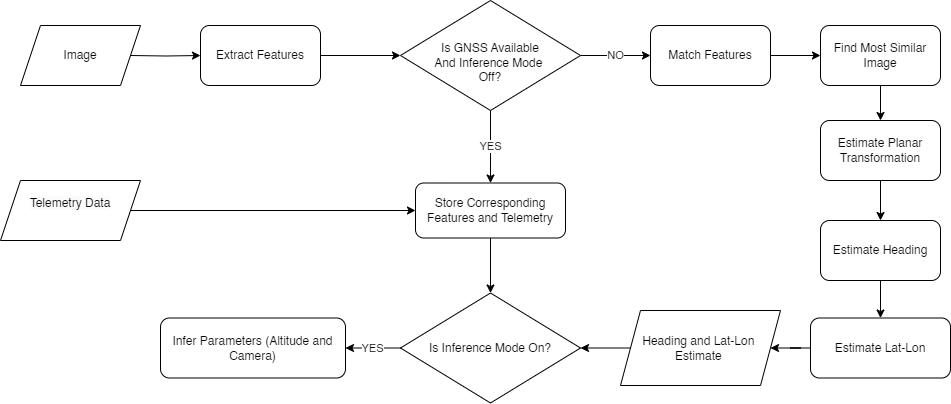
\includegraphics[width=0.99\textwidth]{Chapter 3/Chap3Figs/HighLevelFlow.png}
    \caption{High-Level Flow of the System}
    \label{fig:HighLevelFlow}
\end{figure}




\section{System Pipeline}
The system pipeline consists of multiple stages, each designed to perform a specific task in the navigation process. The pipeline is designed to be robust, accurate, and computationally efficient, ensuring reliable navigation in various operational scenarios. The pipeline stages are detailed below.

\subsection{Pipeline Stages}

\begin{enumerate}
    \item \textbf{Image (Input):}  
    The process begins with capturing a live image from the UAV’s downward-facing camera. This real-time visual input provides essential information about the UAV’s environment, forming the basis for position estimation.

    \item \textbf{Extract and Store Features:}  
    Keypoints and descriptors are extracted from the current image to aid in the matching process. This extraction occurs in two layers: the coarse layer, used in the second stage of image match search space reduction, and the dense layer, used during the precise transformation stage. The system also extracts features when GNSS is available to reduce computational load during critical phases when GNSS is lost.
    
    \item \textbf{Store Corresponding Features and Telemetry:}  
    Extracted features (keypoints and descriptors) along with their corresponding telemetry data (GNSS position and heading) are stored for future reference. Stored features facilitate relative transformation inference when GNSS is unavailable, while telemetry data assists in converting relative transformations to real-world coordinates and headings.

    \item \textbf{Infer Parameters (Altitude and Camera):}  
    To be able to convert from a pixel translation to a metre value, a conversion factor is required. This conversion factor is dependent on the altitude of the UAV and the camera's focal length. When GNSS signal is available, this stage uses the complete pipeline to estimate the UAV's Lat-Lon coordinates using a placeholder factor value. These estimates are accumulated and compared, using only the first 5 images to balance overall efficiency and parameter accuracy, with the ground truth Lat-Lon coordinates via linear regression to infer the conversion factor. This is necessary in the scope of this study, which assumes constant and unknown altitude and camera parameters. These parameters are both represented within a single factor, the pixel to metre ratio. 

    \item \textbf{Match Features:}  
    Features between the current image and reference images are matched to ensure that comparisons are based on mutual features. This involves matching of both the coarse and dense layers of features.

    The matching process is optimized to ensure robustness against noise and outliers, with a focus on computational efficiency. The techniques include usage of match acquisition techniques, search techniques, as well as subsequent optimization techniques to refine the matches.
    
    \item \textbf{Find Most Similar Image:}  
    The stage involves two layers of potential image match search space reduction until a single image is chosen for the current image to accurately infer its relative transformation against. 
    
    The first is reduction based on proximity to the last known Lat-lon Coordinates. This stage outputs 5 matches. 
    
    Thereafter, a more precise global matching technique is applied to identify the most similar match from the reduced image search space. This requires initial rotational alignment using the coarse layer of matched features and subsequent global matching techniques to identify the best match based on similarity scores. The crude layer is chosen as global matching techniques were proven in the testing phase to be robust against minor rotational inaccuracies, allowing for efficiency prioritization. 


    \item \textbf{Estimate Planar Transformation:}  
    After identifying the best match, the system performs a precise estimation of both rotation and translation between the input and reference images using the dense match layer. 
    
    The first step involves estimating the rotation between the images, followed by aligning the images based on this rotation. 
    
    Thereafter, the system recomputes the dense layer of features and matches on the aligned images. The reason for the recomputation prior to translation estimation is due to improved accuracy; aligned point clouds allow for improved translation estimation by way of less parameters to estimate. The amount of mutual information also remains constant when applying alignment to an image. 

    Finally, the system estimates the translation between the images using the refined dense layer. 

    This rotation and translation estimation are outputted to the next stages for conversion from relative to absolute conversion of the UAV's heading and position. 

    \item \textbf{Estimate Heading:}
    The internal angle between the current and reference images is added to the reference image's heading to determine the UAV's current heading. 
    \item \textbf{Estimate Lat-Lon:}  

    The estimated translation at this stage is a pixel value representing the displacement between aligned images. To convert this to real-world latitude and longitude coordinates, the vector must be scaled in magnitude and rotated to align with the global coordinate system. This process consists of the following steps:

    The translation vector, initially relative to the internal image coordinate system, is rotated by the heading of the reference image, aligning it with the global latitude-longitude system without altering its pixel magnitude.  

    Next, the estimated pixel displacement is multiplied by the inferred pixel-to-metre conversion factor, resulting in a translation vector in metres with East and North components. 

    Then, this vector is converted to a latitude and longitude displacement. To account for the Earth's oblate spheroid shape, the equations below are used, which consider the latitude-dependent distance per degree of longitude:  
    
    $ \Delta \text{Lon} = \frac{\Delta \text{East}_{\text{m}}}{111320 \cdot \cos(\text{Lat}_{\text{ref}})}, \quad \Delta \text{Lat} = \frac{\Delta \text{North}_{\text{m}}}{111320} $

    where the East and North components represent the eastward and northward displacement vector components in metres, aligned to the global coordinate system. The constant 111320 converts degrees of latitude to metres, with longitude scaled by $\cos(\text{Lat}_{\text{ref}})$ to reflect latitude-dependent longitudinal distance. 

    Finally, the calculated displacements in latitude and longitude are added to the reference image’s known coordinates, yielding the UAV’s estimated absolute position.  

    \item \textbf{Heading and Lat-Lon Estimate:}
    The systems heading and Lat-Lon estimates are outputted to the user interface for real-time monitoring and in practice, navigation.


\end{enumerate}


\section{Dynamic Methods and Techniques}
Testing showed that the degree of environmental variation often leads to situations where a static pipeline will either not find a sufficient number of matches or take too long. To maintain generalizability across datasets (terrains), adaptive methods were implemented to adjust the pipeline without prior knowledge of the environment.

The first adaptation was made to AKAZE, which did not have a built-in method to adjust the number of keypoints detected. This method sampled the first image in the dataset and altered its threshold iteratively until a set number of keypoints were found. This was done once per dataset to maintain computational efficiency, but in practice, it may be done per n images or per time interval.

Secondly, Lowe's ratio employed an adjusting threshold that increased in leniency until a set number of matches or a percentage of available keypoints were found. This was done per image.


\section{Testing Shortlist}
\label{sec:testing_shortlist}
The following methods and techniques were tested, with some exclusions based on empirical results:

\textbf{Feature Detectors:} AKAZE, SuperPoint (with LightGlue matcher), and ORB. Note, the SuperPoint detector is used in conjunction with the LightGlue matcher to enhance performance.

\textbf{Feature Matchers:} FLANN and BruteForce. KNN.

\textbf{Search Techniques:} KNN with \( K=2 \). Empirical tests showed a value of 1 to be ineffective since it excluded Lowe's ratio test, while values above 2 introduced excessive computational overheads. Further, radius search was seen to be unreliable due to the varying density of keypoints across datasets.

\textbf{Planar Transformation Estimation:} Homography, Affine, Partial Affine (Rigid) transformations using OpenCV, and SVD-based rigid transformations for rotation and translation estimations. Rotational and translational estimates were initially tested separately, due to the possibility of different responses to different prior stages and methods. However, it was seen that inter-method comparisons subtended equivalent conclusions; the methods were tested for visual brevity using a combined transform.

\textbf{Global Image Similarity Measures:} SSIM, histogram matching, local retrofit, and cross-correlation.

\textbf{Optimization Techniques:} Standard Deviation Filtering, LMEDS, RANSAC, Lowe's ratio test, n-Match thresholding, and absolute thresholding for match refinement. Empirical tests indicated that cross-checking was not applicable due to the excessive computational costs involved. KNN.


\section{Software}
This sections details a snippet from the main loop showing the key software flow. 

The full code may be found at \url{https://github.com/Samshabz/Skripsie}

\begin{lstlisting}[language=Python, basicstyle=\ttfamily, keywordstyle=\bfseries, commentstyle=\itshape\color{gray}]
    
# Setup Lines...

# Phase 1: GNSS is Available and Inference Mode is On
for i in range(1, inference_images + 1): 
    navigator.add_image(i, directory)
navigator.estim_pos(inference_images, Inference_Mode_On=True)
navigator.find_pixel_to_metre_factor()

# Phase 2: GNSS is Available and Inference Mode is Off
for i in range(inference_images+1, total_images + 1):
    navigator.add_image(i, directory)

# Phase 3: GNSS is Unavailable
navigator.estim_pos(total_images, Inference_Mode_On=False)

# Debug Lines...

\end{lstlisting}





